\section{Methodology}

This section will describe the methodology to fulfill the research target. As mentioned in the \ref{aor}, the primary goal of this research is to introduce the bayesian learning method into active learning framework to handling the learning problem with variant size of data set and enable the model flexible enough to adapt the model complexity. 
\begin{figure}[htbp]
\centering
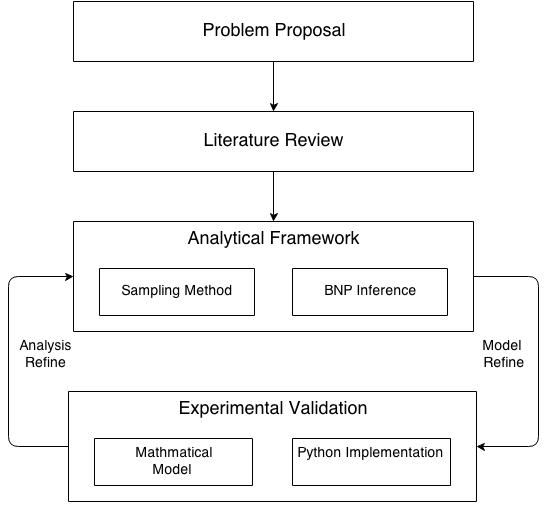
\includegraphics[width=\linewidth]{proposal}
\caption{Research Flowchart}
\label{fig:proposal}
\end{figure}

Fig\ref{fig:proposal} is the main flowchart.  briefing the detailed process, and in each main stage the major work should be:
\begin{enumerate}
 \item \textbf{Literature Review}
 
 This part contains a comprehensive review on the machine learning literature, especially on the relevant topics in this proposal. Besides the classical learning theories, extensive reading on analysis of their characteristics and application should also be focused on. The goal is to gain a general understanding of the theory framework, relation to other learning theory,  their history, development and current research. 
 
 \item \textbf{Design a metric learning framework that will support big data set }
 
 Currently, most of the existing distance metric learning approaches involve computationally expensive procedure in which it requires an iterative eigen-decomposition of metric matrix $M$, let alone when it comes to big data set. We are going to design a distributed computation framework to handle the problem. The basic idea is to redesign the original algorithm express to avoid the eigen-value decomposition which require expensive computation. 
 
 We plan to design a distributed framework that implements parallel DML. Based on the Bayesian Nonparametric method, we partition the data onto different nodes. Each nodes uses the data it hods to update the model parameters to gain a local optimum. The challenge is the synchronization of the parameters trained on each nodes. We plan to use a central node to synchronize the parameters across machines.
 
 \item \textbf{Propose a new Gibbs Sampling method to accelerate the convergency in DPMM}
 
 As shown in literature review, traditional Gibbs sampling in Dirichlet process mixture model demonstrate a low convergency, especially when applying on a large data set since the sampler will traverse all the observations to get the parameters updated according to the posterior distribution. Though several methods has been proposed by a representation of the basic DPMM model, such as introducing split-merge model to improve the probability of generating new cluster, super cluster and sub-cluster to make parallel computing possible to this framework. But this focuses on the sampling the procedure leaving the original data set intact. In order to overcome the curse of large data set, we are trying to propose a method that including a high quality preprocessing of the data set according to a criterion coupling with the sampling process. This idea is motivated by the shema of Active Learning theory. 
 
 We plan to avoid the slow convergency rate caused by the size of data set by selecting a subset of the original observations as a initial training set and during the sampling procedure if a new cluster is generated we will jump into a procedure  selecting observations that will support the new cluster. The first key point in this algorithm is to design a new criterion function and second one is to expolore whether the bias of the initial training set will affect the final training result.
 
 \item \textbf{Metric Learning on multi-modal problem}
 
 Currently, the metric learning problem is mostly applied on the single modality problem and for multi-modal problem, it required further research. McFee and Lanckriet\cite{McFee2011} proposed a kernel-learning methods. But it is computationally costly because it involves optimizing over multiple high-dimensional positive semi-definite matrices and it is hard to scale to large date set. Another piece of work by \cite{Chen2010} integrates multi-wing harmonium model and large margin learning to predictively learn a latent subspace for multi-view data by using the class labels.
 
 We plan to propose a general supervised framewok of multi-modal distrance metric learning methods which can flexibly embed arbitrary number of features modalities using the "similar" and "sissimilar" pairs.
 \item \textbf{Implementation and Experiment}
 
 This steps include implementing the proposed framework and test the algorithm on different data set regarding the specific problem this framework will be used to evaluate its performance. The validation should contain two stage, the first one being comparison with classical and state-of-art algorithm in active learning and bayesian nonparametric model leanring respectively, the second one being test the performance of the whole framework.
 
 
 The result will be compared to the state-of-art methods,in the area of the problem to be solved, such as classification, regression or density estimation, on the basis of both the efficiency and accuracy. The accuracy is to test how our proposed method performs regarding to the specific target of the problem. And the efficiency is to check whether this framework will decrease the rely on calculation resource, both time and space. The performance will be the feedback for analytical refinement.
\end{enumerate}